\jxhj{%教学后记
	}
\skrq{%授课日期
	2018年1月9日 4-5节}
\ktmq{%课题名称
	 变量编程概述}
\jxmb{%教学目标,每行前面要加 \item
	\item 掌握变量的概念;
	\item 掌握变量的赋值与引用;
	\item 理解变量的分类;
	\item 灵活使用变量。
}
\jxzd{%教学重点,每行前面要加 \item
	\item 掌握变量的赋值与引用;
	\item 理解变量的分类。 }
\jxnd{%教学难点,每行前面要加 \item
	\item 灵活使用变量。 }
\jjff{%教学方法
	通过讲述、举例、演示法来说明;}

\makeshouye %制作教案首页

%%%%教学内容
\subsection{组织教学}
\begin{enumerate}[\hspace{2em}1、]
	\item 集中学生注意力;
	\item 清查学生人数;
	\item 维持课堂纪律;
\end{enumerate}

\subsection{复习导入及主要内容}
\begin{enumerate}[1、]
\item Fanuc指令格式;
\item Sienes指令格式;
\item 编程实例。
\end{enumerate}

\subsection{教学内容及过程}
	
\subsubsection{变量与常量}

	常量:指其值不变的量。如数值:1、4、6
	
	字符: “A”、”b”
	
	布尔值:”TURE”、”FALSE”
	
	变量:由变量名(变量号)和变量值组成,其值可以改变,
	
	变量就是指其值可以改变的量。
	
	分析:程序结构相同,如果使用变量,则两个程序可以合为一个程序。
	
	长 宽 圆弧半径 深度等 都可以使用变量

	可以用表达式来指定变量。
	
\subsubsection{Fanuc上的变量}

	1、变量号(变量名)

	$\#$1-\#33   \#100-\#199  \#500-\#999  \#1000以上

	由变量符号”\#”和后面的变量号组成。

	2. 变量的赋值:

	赋值是指将一个数据赋予一个变量

	A . 在程序中赋值:

	\#1=10      \#2=5+5       \#3=\#3+1  \#5=\#7

	注意: ”=”为赋值号, 并等于号

	赋值号”=”两内容不能随意互换, 左边只能是变量, 而右边可有是表达式, 数值或变量.

	一个赋值语句只能给一个变量赋值.

	可以多次给一个变量赋值, 新变量值将取代原变量值. 

	赋值表达式的运算顺序与数学运算顺序相同

	B. 在宏程序调用指令中赋值:(不讲)

	如 G66 P5000 A10.0 B11.0

	A10.0 B11.0 会给5000号宏程序中的\#1, \#2 赋值

	宏调用中的A B C 与 \#1 \#2… \#20有一种邦定关系.

	C. 在系统参数中设定变量的值:

	Fanuc中操作如下: 

	Offset-----[下一页]-------[Macro]

	\#1--\#33   \#100--\#199   \#500--\#999

	3、变量值的范围及小数点

	10-29-1047

	定义变量时,整数值的小数点可以省略。

	如:\#100=123   变量\#100的值为123.000

	4. 变量值的引用

	在程序中使用变量时, 在相应的字后跟上变量号即可. 当用表达式指定变量时, 必须把表达式放在括号中, 如

	G1 X\#1 Y\#2

	G1 X[-\#1-10] 


	改变变量的符号, 可直接在\#前面加”-“, 如 G1 X-\#1

	注意: O N G L P / 后不能使用变量.

	程序的修改。

\subsubsection{变量的分类}

	系统变量, 用于系统内部运算时各种数据的存储. \#1000以上,如刀具当前位置和补偿值等.

	用户变量, 包括局部变量与公共变量, 用户可以单独使用, 系统作为处理资料的一部分.

	局部变量: \#1-\#33 , 只能在宏程序中存储数据, 例如运算结果, 断电
	时,局部变量清除(初始值为空)

	公共变量: \#100-\#199(数据断电清除)

	\#500-\#999(数据断电时也不会清除)

	公共变量在不同的宏程序中意义相同(即公共变量对于主程序和从这些主程序调用的每一个宏程序来说是公用的.)

	举例说明:  个人的钱包   局部的

	班上的班费   公共的

	实例程序的修改:讲解

\subsubsection{算术}

	1. 加减乘除:

	\#i=\#j+\#k           \#i=\#j-\#k
	
\#i=\#j*\#k           \#i=\#j/\#k

2.三角函数:

\#i=SIN[\#j]          \#i=COS[\#j]

\#i=ASIN[\#j]         \#i=ACOS[\#j]

\#i=TAN[\#j]         \#i=ATAN[\#j]/[\#k] (可理解为对边/邻边)

注意: 三角函数及反三角函数的数值均以度为单位来指定

如90度30分应表示为90.5度

3.开平方根,舍入,绝对值:

\#i=SQRT[\#j]        \#i=ABS[\#j]

\#i=ROUND[\#j]

4.指数对数

\#i=EXP[\#j]

\#i=LN[\#j]

5.取整

上取整  \#i=FIX[\#j]

下取整  \#i=FUP[\#j]

\subsubsection{运算顺序与括号}

略

\subsubsection{加工实例}

\begin{figure}[h]
	\centering
	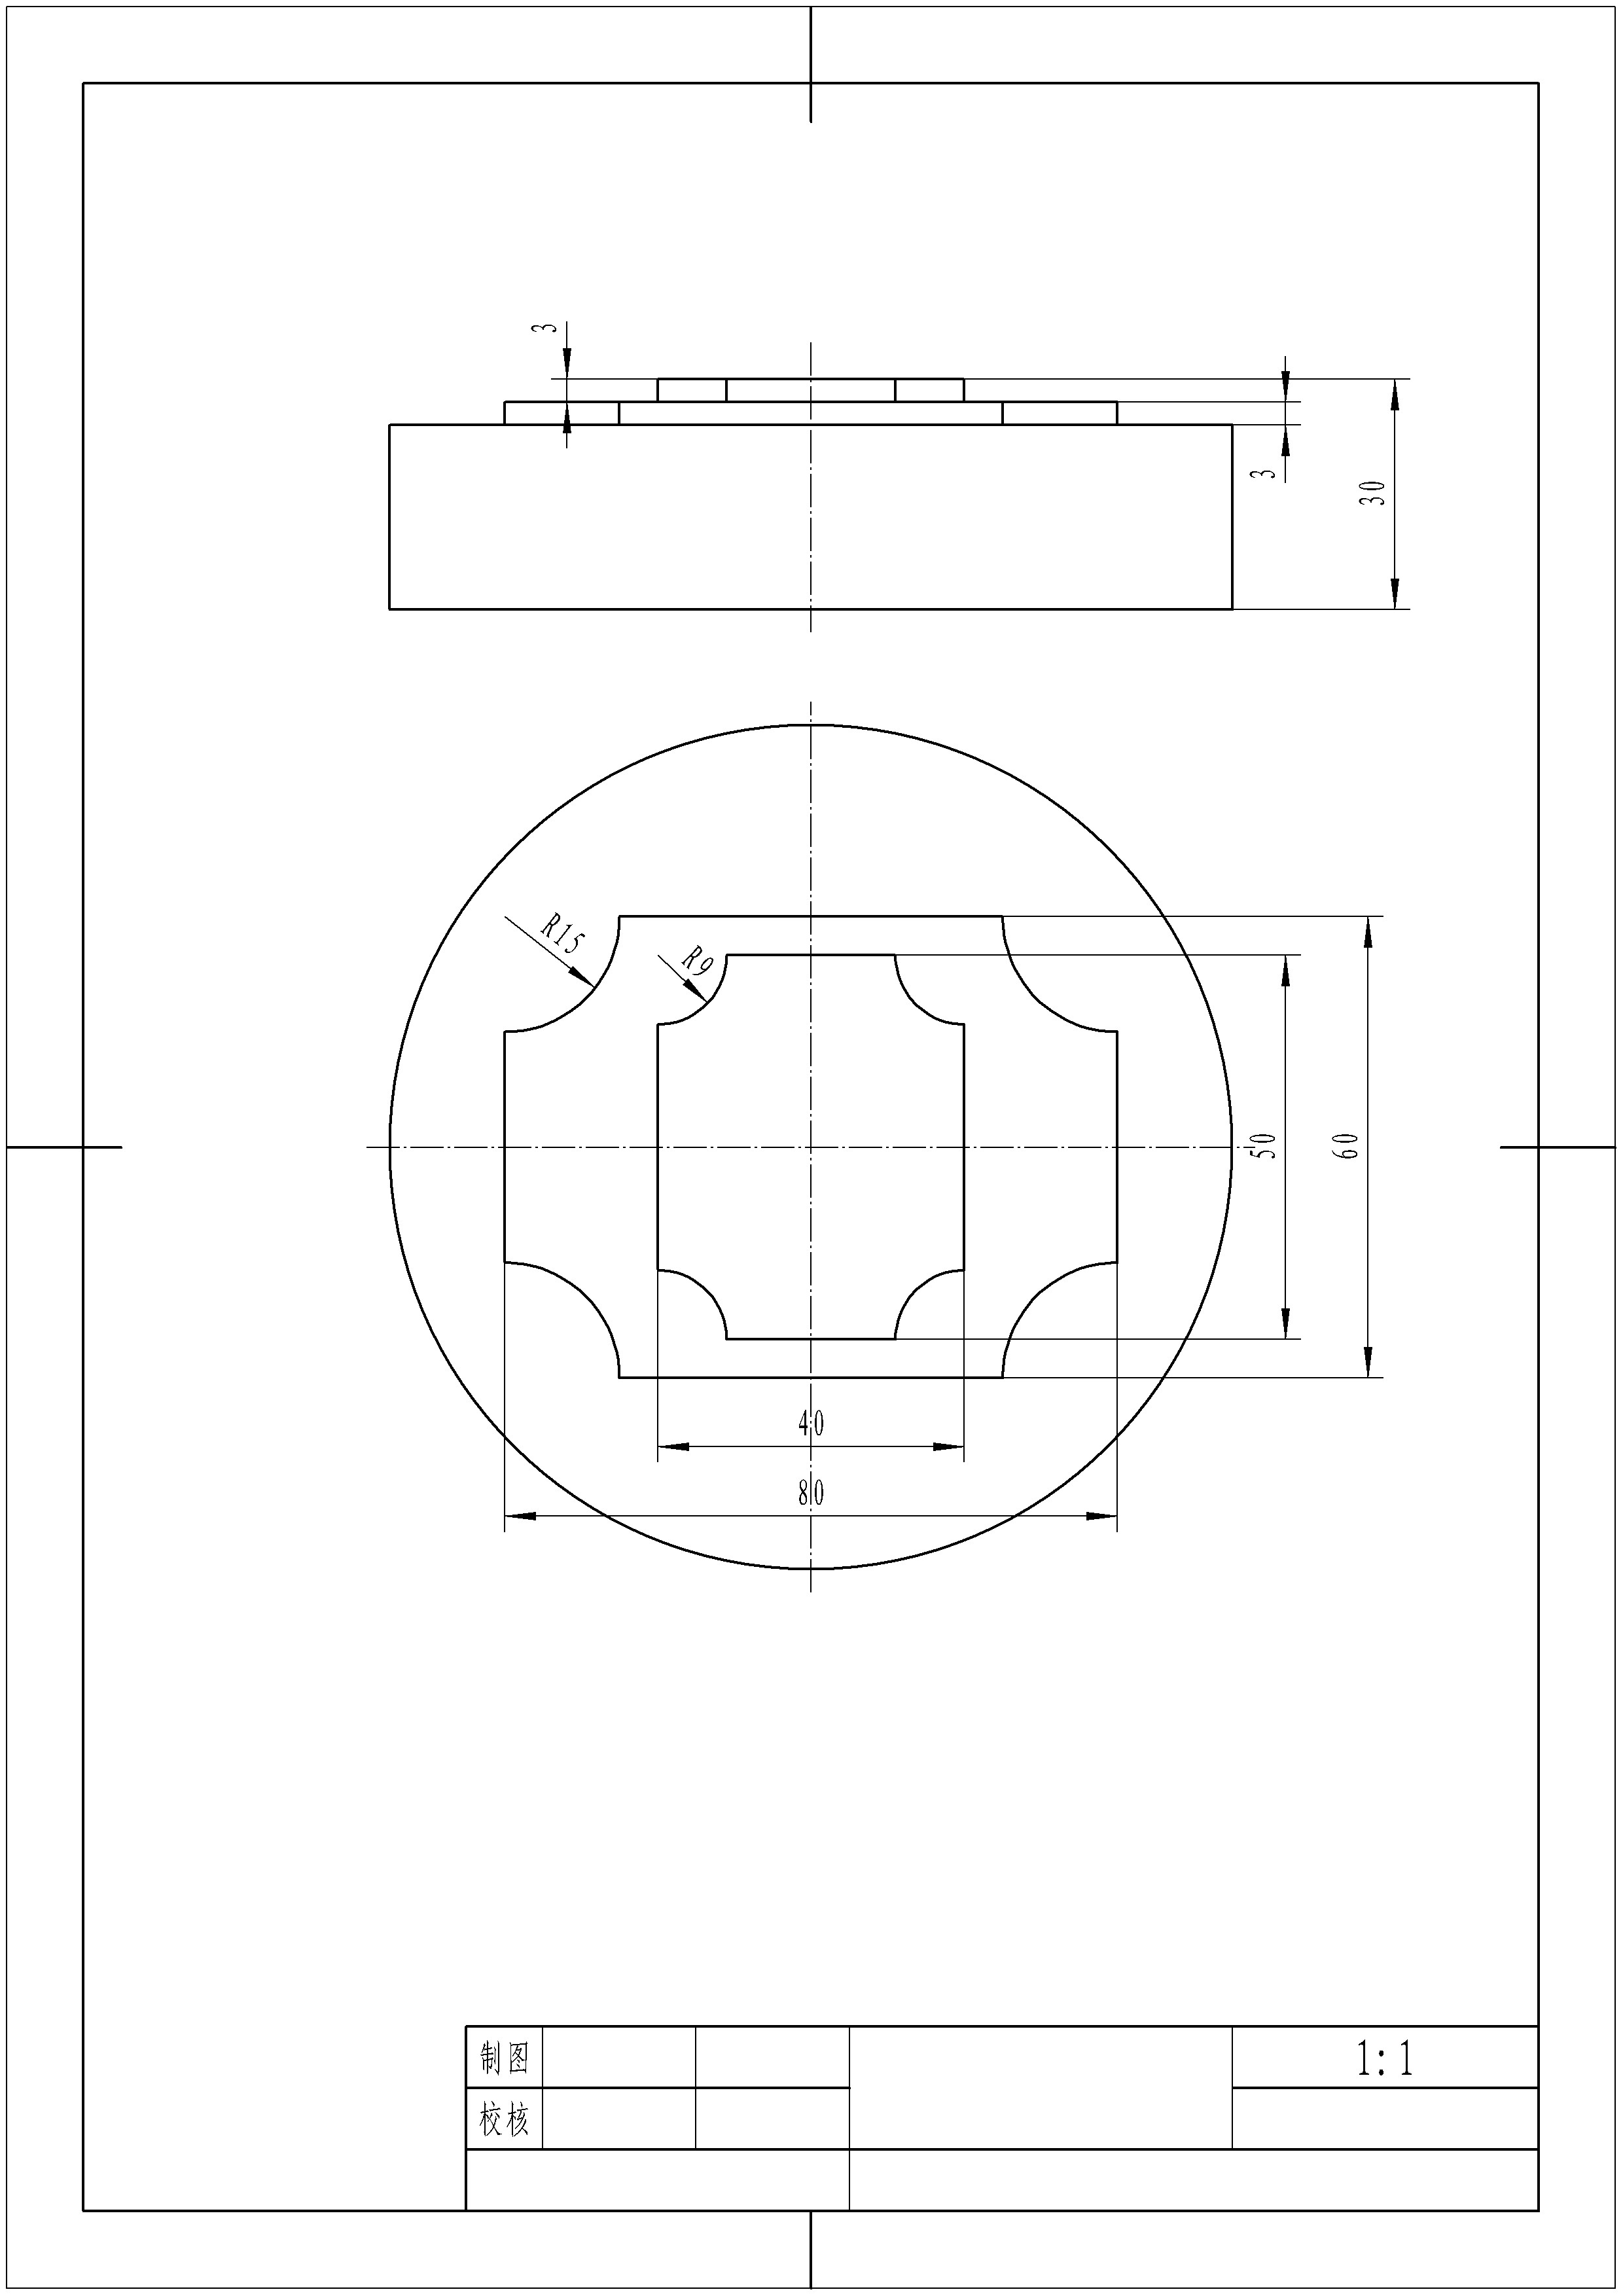
\includegraphics[width=0.7\linewidth,trim=0 0 0 0,clip]{data/image/33-1}
	\caption{加工实例}
	\label{fig:33-1}
\end{figure}

\subsection{课堂小结}
\begin{enumerate}[1、]
\item 变量与常量;
\item Fanuc上的变量;
\item 变量的分类;
\item 算数运算;
\item 运算顺序与括号;
\item 加工实例。
\end{enumerate}

\vfill
\subsection{布置作业}
\begin{enumerate}[1、]
	\item 综合习题一。
\end{enumerate}
\vfill